\documentclass{article}

\usepackage{tikz}
\usetikzlibrary{graphs.standard, quotes}
\usepackage{amsthm}
\usepackage{enumitem}
\usepackage{mathtools}

\title{CSCI 570 - Fall 2021 - HW 8}
\author{Shangning Xu}

\begin{document}

\maketitle

\section*{Graded}

\begin{enumerate}
    \item
    \begin{enumerate}
        \item Refer to Figure~\ref{fig:1a}.
        \begin{figure}[ht]
            \centering
            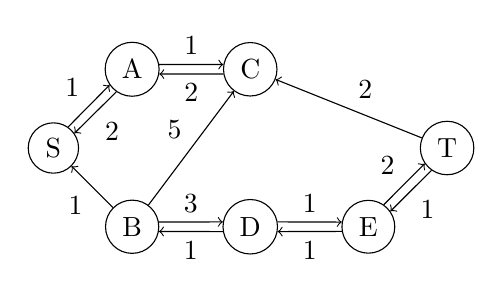
\begin{tikzpicture}
                \foreach \position / \label in {(0, 1)/S, (1, 2)/A, (1, 0)/B, (2.5, 2)/C, (2.5, 0)/D, (4, 0)/E, (5, 1)/T}
                    \node (\label) at \position [circle, draw] {\label};
                
                \draw [->] (node cs: name=S, angle=55) -- node [above left] {1} (node cs: name=A, angle=-145);
                \draw [->] (node cs: name=A, angle=-125) -- node [below right] {2} (node cs: name=S, angle=35);
                
                \draw [->] (B) -- node [below left] {1} (S);
            
                \draw [->] (node cs: name=A, angle=10) -- node [above] {1} (node cs: name=C, angle=170);
                \draw [->] (node cs: name=C, angle=-170) -- node [below] {2} (node cs: name=A, angle=-10);
            
                \draw [->] (node cs: name=B, angle=10) -- node [above] {3} (node cs: name=D, angle=170);
                \draw [->] (node cs: name=D, angle=-170) -- node [below] {1} (node cs: name=B, angle=-10);
            
                \draw [->] (B) -- node [above left] {5} (C);
            
                \draw [->] (node cs: name=D, angle=10) -- node [above] {1} (node cs: name=E, angle=170);
                \draw [->] (node cs: name=E, angle=-170) -- node [below] {1} (node cs: name=D, angle=-10);
            
                \draw [->] (node cs: name=E, angle=55) -- node [above left] {2} (node cs: name=T, angle=-145);
                \draw [->] (node cs: name=T, angle=-125) -- node [below right] {1} (node cs: name=E, angle=35);
            
                \draw [->] (T) -- node [above right] {2} (C);
            \end{tikzpicture}
            \caption{Residual graph for Question 1 (a)}
            \label{fig:1a}
        \end{figure}
        
        \item The max-flow value is 3. The minimum cut is $(\{S, A, C\}, \{B, D, E, T\})$.
    \end{enumerate}

    \item
    \begin{enumerate}
        \item We define the corresponding flow network to an instance of the given problem as follows:
        \begin{enumerate}
            \item One vertex for each student and class, with an additional source and sink vertices.
            \item Add an edge between each student and the source with capacity $m$.
            \item Add an edge between each class $c_j$ and the sink with capacity $q_j$.
            \item Add an edge between each student $s_j$ and classes they want to sign up for with unit capacity.
        \end{enumerate}

        Our algorithm runs the Ford-Fulkerson method over the flow network to obtain a maximum flow. If the maximum flow value is exactly $mn$, then all students can be enrolled as full-time students.

        To prove the correctness of our algorithm, we first lay out some definition. We define a \emph{valid enrollment} to be a set of student-course pairs $(s_i, c_j)$ such that student $s_i$ is enrolled in class $c_j$ where the number of students enrolled in a class is within the class's capacity. Let $n_i$ be the number of classes student $s_i$ enrolled in and $m_i$ be the number of students enrolled in class $c_i$.
        
        First, we prove the following proposition: there is a valid enrollment of size $N$ if and only if there is an integer-valued flow $f$ in the corresponding flow network such that $|f| = N$.
        \begin{proof}
            \begin{description}
                \item[$\implies$]: If there is a valid enrollment, define the flow $f$ as follows:
                \[
                    f(u, v) = \begin{dcases*}
                        n_i & if $u = s$ and $v = s_i$,\\
                        1 & if student $u$ is enrolled in class $v$,\\
                        m_i & if $u = c_i$ and $v = t$,\\
                        0 & otherwise.
                    \end{dcases*}
                \]

                One can easily verify that $f$ satisfy capacity constraint and flow conservation. The flow across the cut $(\{s\}, E - \{s\})$ is $\sum_{i = 1}^n n_i = N = |f|$.

                \item[$\impliedby$]: Given an integer-valued flow $f$, define the valid enrollment to be $\{(s_i, c_j)| f(s_i, c_j) > 0\}$. For any vertex $s_i$, $f(s, s_i) < p_i$ is exactly the number of classes student $s_i$ enrolled in due to flow conservation, and $f(c_i, t) < q_i$ is the number of students in class by the same argument. Therefore, the enrollment induced by flow $f$ is valid and the total number of classes all students enrolled in is exactly $N = \sum_{i = 1}^n f(s, s_i) = |f|$.
            \end{description}
        \end{proof}

        Then, if there exists an integer-valued flow $f$ whose value is $mn$, then the size of enrollment induced by $f$ is $mn$ and every student is a full-time student as they are enrolled in exactly $m$ classes, as mandated by the cut $(s, V - \{s\})$. Because the cut $(s, V - \{s\})$ has capacity $mn$, a flow of value $mn$ is also a maximum flow.

        \item We tweak the flow network in (a) by removing edges between students and classes when the student is not enrolled in the class, change capacity of edges between source and students to $r$ and capacity of edges between classes and sink to 1. We solve for the maximum flow value on the new flow network. If the flow value is exactly the number of classes, then the required selection exists.
        
        The prove of correctness of our algorithm is similar to the one in (a).
    \end{enumerate}

    \item
    \begin{enumerate}
        \item False. Consider the following flow network. After replacing the edges, the edge $(s, t)$ is added, allowing a maximum flow with value 100.
        \begin{center}
            \tikz \graph [math nodes] {
                subgraph I_n [V={v, t, s}, clockwise, nodes={draw, circle}];
                s -> ["1"] v -> ["1"] t -> ["100"] s;
            };
        \end{center}

        \item False. The edge $(x, t)$ is present in two scaling phases.
        \begin{center}
            \tikz \graph [math nodes, nodes={draw, circle}] {
                subgraph I_n [V={v, x, u, s}, clockwise];
                s -> ["8"] v -> ["6"] x -> ["10"] t [right of=x];
                s -> ["2"] u -> ["2"] x;
            };
        \end{center}

        \item True.
        \begin{proof}
            After all edges are multiplied by $k$, for any cut $(S, T)$ of the flow network, its new capacity
            \[
                c'(S, T) = \sum_{u \in S} \sum_{v \in T} kc(u, v) = k \sum_{u \in S} \sum_{v \in T} c(u, v) = kc(S, T).
            \]

            Because cut capacities are all positive, after multiplied by $k$, the original minimum cut's capacity remains minimum among all cuts.
        \end{proof}

        \item False. Consider the following flow network. After increasing edge capacities, the maximum flow increases from 2 to $4 > 3$.
        \begin{center}
            \tikz \graph [math nodes, edge label=1] {
                subgraph I_n [V={v, t, s}, clockwise, nodes={draw, circle}];
                s -> v -> t;
                s -> t;
            };
        \end{center}
    \end{enumerate}

    \item To decrease the maximum flow by as much as possible by deleting at most $k$ edges, find a minimum cut in the flow network and delete $k$ (or as many as possible) edges from the cut. The algorithm runs in polynomial time as a minimum cut can be found in polynomial time, and deleting edges takes linear time.

    When not all edges have unit capacities, our algorithm doesn't guarantee that the maximum flow is decreased by as much as possible. Consider the following graph with $k = 2$ as an example:
    \begin{center}
        \tikz \graph [math nodes, nodes={draw, circle}] {
            s -> ["2" above] {a -> ["1"] c, b -> ["1"] t};
            a -> ["1" above] t;
            c -> ["1"] t;
        };
    \end{center}
\end{enumerate}

\section*{Ungraded}

\begin{enumerate}[resume]
    \item We define the corresponding flow network to an instance of the given problem as follows:
    \begin{enumerate}
        \item Add a vertex for every tourist and every currency, along with a source and sink.
        \item Add an edge between the source and each tourist $t_k$ with capacity $F_k$, an edge between each currency $c_j$ and the sink with capacity $B_j$ and an edge between $t_k$ and $c_j$ with capacity $S_{kj}$.
    \end{enumerate}

    We run the Ford-Fulkerson method on the flow network to obtain a maximum flow. If the maximum flow value is exactly $\sum_{k = 1}^n F_k$, then all tourists' requests can be fulfilled.

    \item We define the corresponding flow network to an instance of the given problem as follows:
    \begin{enumerate}
        \item Add a source and connect it to each entrance. Add a sink and connect each exit to it.
        \item Split each vertex $v$ that is neither an entrance nor an exit into two vertices $v_\textrm{in}$ and $v_\textrm{out}$ with edge $(v_\textrm{in}, v_\textrm{out})$. Connect $v$'s incoming edges to $v_\textrm{in}$ and outgoing edges to $v_\textrm{out}$.
        \item Assign unit capacity to each edge.
    \end{enumerate}

    We run the Ford-Fulkerson method on the flow network to obtain a maximum flow. If the maximum flow value is exactly $k$, then there exists an arrangement for the private showings where no client will see each other. Proof correctness for our algorithm is similar to the one in Question 2 (a).

    \item By Kőnig's theorem, the number of edges in a maximum matching equals the number of vertices in a minimum vertex cover in any bipartite graph. Therefore, we just need to find a maximum matching in the bipartite graph with maximum flow algorithm. The graph has a vertex cover of at most size $k$ if and only if the value of the maximum flow is not greater than $k$.
\end{enumerate}

\end{document}
